\documentclass{article}
%\documentstyle[aps]{revtex}

%\usepackage{enumerate}


%\newcommand{\hode}[1]{ \vspace*{0.3cm}
%                       \noindent
%                       {\sc #1}\\[-0.3cm]
%                       \rule{\textwidth}{0.3mm}\\   %[0.2cm]
%                     } 
 
%\newcommand{\vjump}{ \vspace*{0.3cm}\\}
\usepackage{amsmath}
\usepackage{graphicx}
\usepackage[latin1]{inputenc} 
%\usepackage[norsk]{babel}
\usepackage{subfigure}



\begin{document}


\begin{center}
  {\bf \Large Project assignment AST2210 -- \\\LARGE Analysis of four-year COBE-DMR data}\\\vspace*{5mm}
  {Hans Kristian Eriksen and Tone Melv{\ae}r Ruud}
\end{center}
\vspace*{15mm}

\section{Introduction}

We will in this project assignment repeat the analysis of the
four-year COBE-DMR observations that were published in 1994, and we
will focus on the two important cosmological parameters, $Q$ and $n$,
corresponding to the \emph{amplitude} and \emph{tilt} of the CMB
spectrum. The analysis is to be described in the form of an
Astrophyiscal Journal Letters (ApJL) paper, and it is this paper that
will be the final product of the project.

Before starting the work, it might be a good idea to read the paper by
G{\'o}rski et al.\ (1994), which is available in the directory
``$\sim$hke/AST2210/cobe\_project'' -- you will more or less
plagiarize this paper :-) All data and program files are also
available in the same directory. 

It might also be worth reading the paper by  Eriksen et
al. (2007) that is available in the same directory, since that has a
structure that is closer to the one you will use. While G{\'o}rski et
al.\ (1994) had a companion paper that described the methods, you will
describe both method, data and results in the same paper. Eriksen et
al.\ (2007) is an example of this structure, with a topic that is
closely related to the current project. 

\subsection{The Cosmic Microwave Background (CMB)}
In this project we will consider observations of the so-called cosmic
microwave background (CMB). Before we start the analysis of these
data, it is a good idea to understand what this is, and we therefore
provide a quick summary here:

The CMB consists of the oldest photons in the universe. These photons
were released about 380\,000 years after the Big Bang. Before that
time, the universe was too hot and dense for electrons and protons to
form neutral hydrogen, and all space was therefore filled with a
plasma of free electrons and protons. In such a gas, photons are
effectively trapped within the plasma, due to frequent
scattering. However, once the temperature fell below 3000K, the
photons were no longer sufficiently energetic to ionize
hydrogen. At this particular time in the history of the universe,
suddenly all free electrons effectively disappeared, merging with
protons into hydrogen, and the photons were free to move throughout
the universe without additional scattering.

Originally, these photons had a temperature of about 3000K. However,
because of the expansion of the universe, the wavelength of these
photons is also stretched. Furthermore, since the universe has
expanded by a factor of about 1100 since that time, the effective CMB
photon temperature is today about 2.7K. The wavelength of such cool
radiation corresponds to microwaves, and it today is observable at
radio frequencies.

Today we can detect this radiation essentially using a very fancy TV
antenna, and measure its intensity in different directions on the
sky. The stronger the intensity, the hotter the photons. And the
hotter the photons, the higher the density was at the time when they
were released. Therefore, a CMB picture corresponds to a ``baby
picture'' of the universe: It shows where the matter density was high
and low shortly after the Big Bang.


\subsubsection{The spherical harmonic decomposition and angular power spectrum}

To analyze this radiation, we need a few useful mathematical tools. As
outlined above, our main concern is the variation in the CMB
temperature as a function of sky position. In order to understand the
statistical properties of these fluctuations, we will need the
spherical harmonic decomposition. Spherical harmonics, $Y_{\ell m}$,
are spherical wave functions. They form a complete basis on the
sphere, and are therefore widely used in all fields of physics. For
instance, you may already have encountered these in quantum physics,
when modelling the hydrogen atom.

The spherical harmonic decomposition corresponds to a spherical
equivalent of the Fourier transform,
\begin{equation}
\Delta T(\hat{n}) = \sum_{\ell = 0}^{\ell_{\textrm{max}}} \sum_{m = -\ell}^{\ell}a_{\ell m} Y_{\ell m}(\hat{n}),
\label{eq:skydecomp}
\end{equation}
where the $a_{\ell m}$-s are wave mode amplitudes describing the
strength of each individual wave length. Each mode is described by two
characteristic numbers, $\ell$ and $m$, where the first quantifies the
effective wavelength of the mode and the latter describes the phase
(or morphology) of the mode.

One can show that for a statistically isotropic and homogeneous field
(ie., a field that is supposed to look statistically the same in all
directions and from all places), there is no important information
carried in the $m$ quantity: The field is essentially just noise. The
important thing is instead simply the \emph{amplitude} of the signal
as a function of wavelength, or equivalently, it's variance. This is
called the \emph{angular power spectrum}, and is defined as
\begin{equation}
\left<a_{\ell m} a_{\ell' m'}^*\right> = \delta_{\ell\ell'}\delta_{m m'} C_{\ell}.
\end{equation}
You will learn much more about this in Cosmology 2, if you choose to
continue with cosmology, where you will learn how to predict this from
first principles.

It is the power spectrum that ties together theory and observations,
in that different models for the evolution of the universe predicts
different shapes and amplitudes for the function $C_{\ell}$. By
comparing those predictions to that measured from the real CMB sky, we
can determine which models fit best with the real universe.

\section{Maximum likelihood analysis of COBE-DMR}

\subsection{Data description}

COBE ({\em COsmic Background Explorer}) was launched by NASA in 1989
to measure the CMB with unprecedented detail. The two most striking
results from this experiment were, first,  its measurements of the CMB
intensity spectrum, which followed a virtually perfect blackbody
spectrum shape, and, second, the first detection of spatial variations
in the CMB temperature. Two of the leaders of the experiment, John
Mather and George Smoot, won the Nobel Prize in Physics for these
discoveries in 2006. 

In this project we will repeat their analysis of the DMR
observations. In particular, we will consider the observations taken
at 53 and 90GHz, corresponding to the two cleanest frequency channels,
ie., those with the lowest noise and least astrophysical foreground
contamination. The 90 GHz map is shown in the top panel of Figure
\ref{fig:map90}.

Next, in order to estimate the variance of the CMB fluctuations, we
first need to know something about the variance of the instrumental
noise. After all, what we will be looking for is essentially an
\emph{excess} variance in the real data above that what is expected
from the instrument. For this, we will assume that the noise per pixel
is Gaussian distributed with zero mean and standard deviation equal to
$\sigma_p$, where $\sigma_p = \sigma_0/\sqrt{N_{obs,p}}$; $\sigma_0$
is the noise per observation, while $N_{obs,p}$ is simply how many
times the instrument has looked at pixel $p$. The values of $\sigma_p$
are tabulated for you. Furthermore, we assume that the noise is
independent between any two pixels, such that the noise covariance
matrix can be written as
\begin{equation}
N_{pp'} = \sigma_p^2 \delta_{pp'}.
\end{equation}

\begin{figure}
\centering
\subfigure{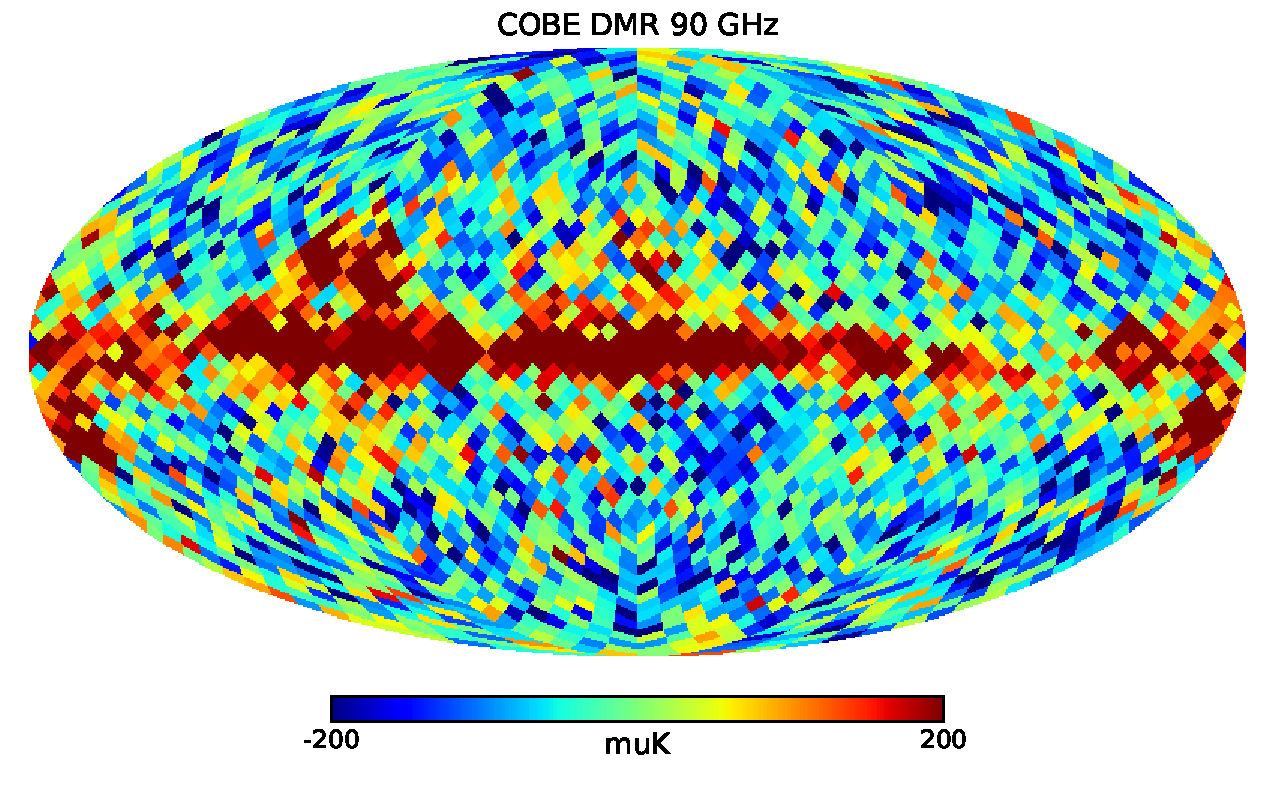
\includegraphics[height=0.3\textheight]{cobe_dmr_map_90GHz_n16.pdf}}
\subfigure{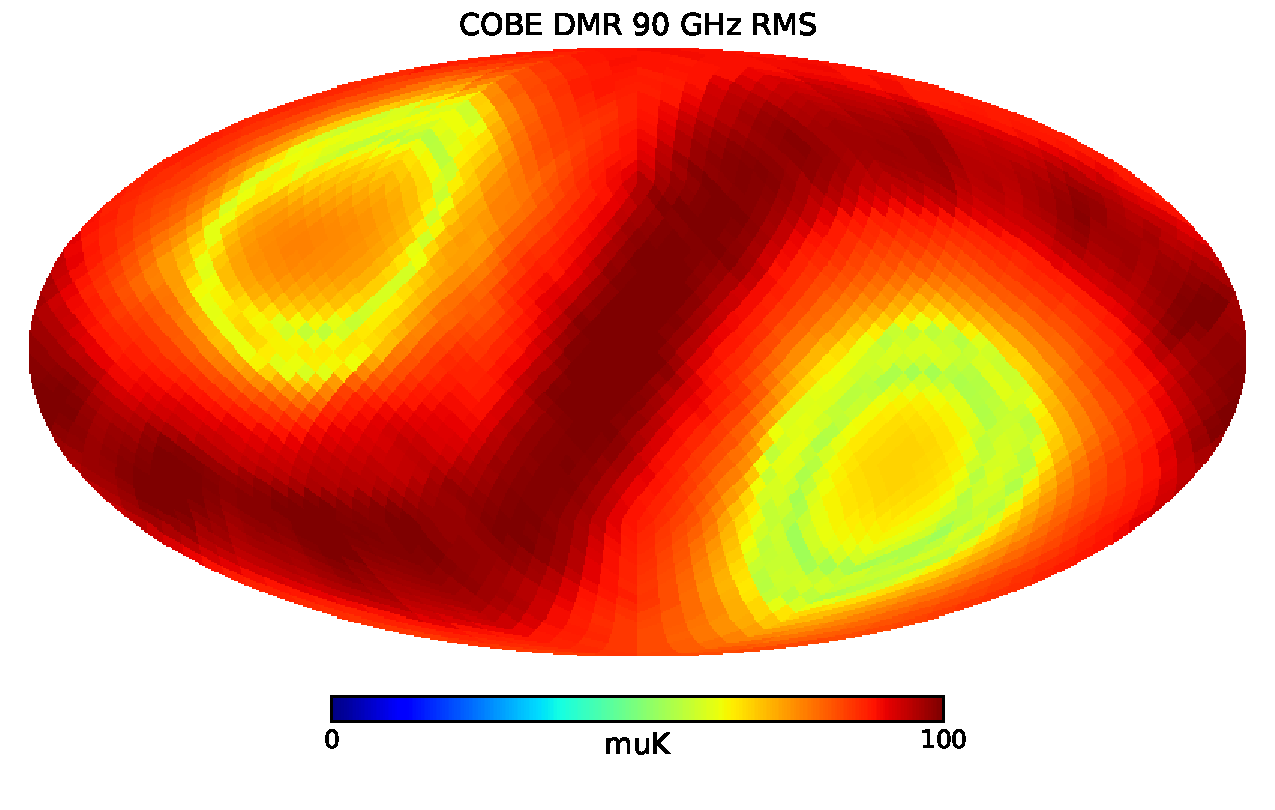
\includegraphics[height=0.3\textheight]{cobe_dmr_rms_90GHz_n16.pdf}}
\caption{Map and corresponding RMS distribution for the COBE-DMR 90
  GHz channel. Note that these maps show the whole sky projected onto
  a plane, using a so-called Mollweide projection. They are shown in
  Galactic coordinates, and the red ``band'' across the top panel
  corresponds to excess foreground radiation from the Milky Way. In
  comparison, the bottom panel shows the effective scanning strategy
  of the COBE satellite, in the sense that where the map is red, the
  noise is high, and the satellite has spent little observation time
  here; where it is yellow, the noise is low, and the satellite has
  spent much time here. The dark red band corresponds to the Ecliptic
  plane, ie., the path of the Sun across the sky during a year. The
  satellite is designed to avoid looking at the Sun, and therefore
  spends less time in this region. \label{fig:map90}}
\end{figure}

As seen in the 90$\,$GHz map, there are some regions of the sky that
are strongly dominated by \emph{foregrounds}. These are strong sources
of radio emission from for instance free electrons or dust grains in
the Milky Way, and they tend to swamp out the CMB signal near the
Galactic plane. To make sure our analysis is not contaminated by this
radiation, we choose to exclude the most contaminated pixels through
the use of a \emph{mask}. This is essentially simply a map consisting
of either 0 or 1's, indicating whether a pixel should be excluded or
not. Figure \ref{fig:mask} shows the mask we will use in this
project. 

\begin{figure}
\centering
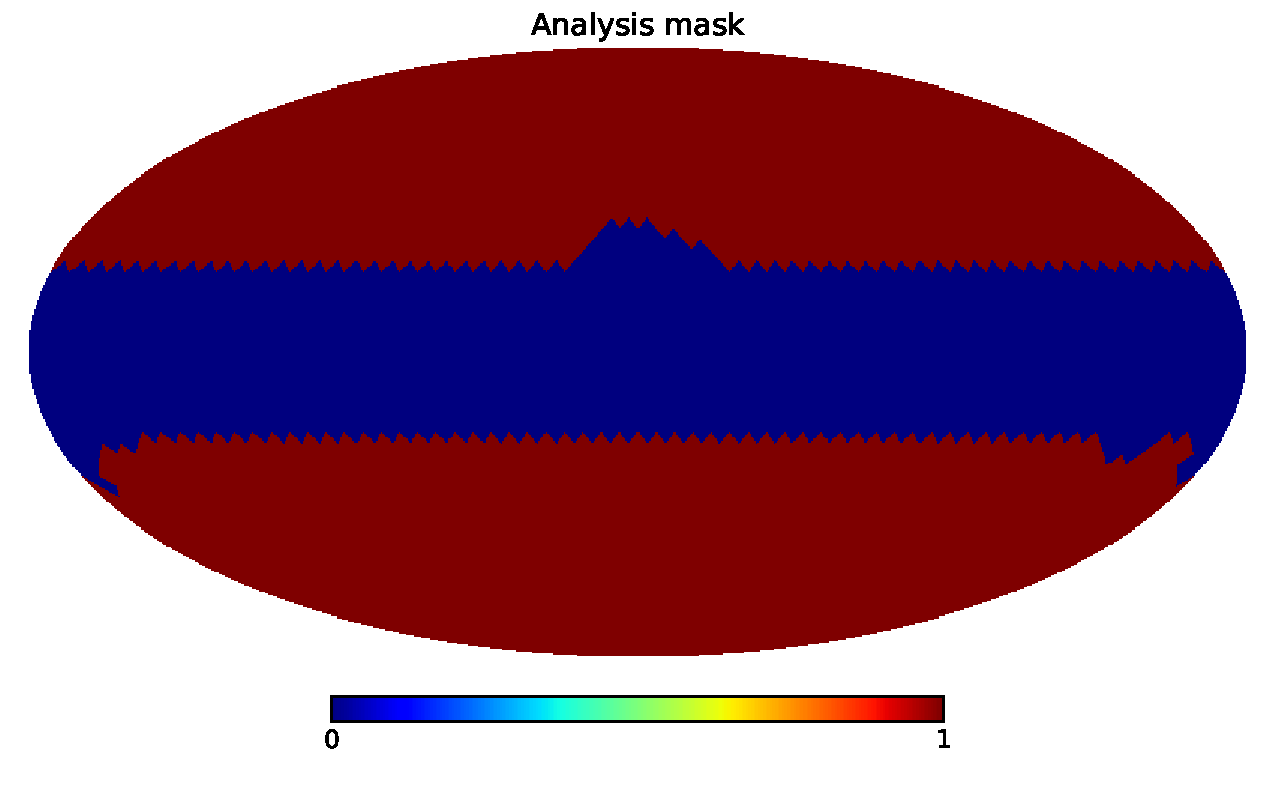
\includegraphics[width=0.6\textwidth]{mask_n16.pdf}
\caption{Analysis mask. The red pixels are included in the analysis,
  whereas the blue pixels hear the Galactic plane are excluded to
  minimize foreground contamination. \label{fig:mask}}
\end{figure}

Next, we have to account for what is called the instrumental
\emph{beam}. This is a function that tells us how large area of the
sky is seen by the instrument at any given time. In optical astronomy
this function is often called the ``point spread function''. At any
given point, the CMB photon bucket that is our CMB telescope will
collect photons from more than one point on the sky. In fact, the
COBE-DMR beam extends 7 degrees (!) on the sky! This beam essentially
corresponds to smoothing the true sky by 7 degrees, thereby
effectively suppressing small angular scales. Mathematically, we can
describe this operation as a convolution in pixel space, which
turn in to a multiplication in harmonic space due to the Fourier
convolution theorem. The net result is that Equation \ref{skydecomp}
is replaced by 
\begin{equation}
\tilde{T}(\hat{n}) = \sum_{\ell = 0}^{\ell_{\textrm{max}}}\sum_{m =
  -\ell}^{\ell} b_{\ell} a_{\ell m} Y_{\ell m}(\hat{n}), \quad\quad
\textrm{beam convolved map}.
\end{equation}
The DMR beam is well known, and we will describe later how to account
for this in the actual analysis. You should also plot it to gain some
intuition for what it means. 

All in all, the DMR data set consists of the following items:
\begin{itemize}
\item Two files with CMB measurements at 53 and 90 GHz, each
  consisting of a total of 1941 data points with associated direction
  vectors. 1131 pixels out of a total of 3072 have been removed by
  masking. The linear size of each pixel is about 220' ($\sim 3.7^{\circ}$)
\item Two associated files containing the variance of each
  pixel, $\sigma_{p}^2$, where $\sigma_{p}$ is given in the files.
\item the instrumental beam, $b_{\ell}$. 
\end{itemize}
These are all available in the directory mentioned above. 
% \begin{itemize}
% \item To CMB-kart observert p� 53 og 90 GHz; pikselisert med
%   $N_{\textrm{side}}=16$, totalt 3072 piksler.
% \item To tilh�rende kart av standard-avviket til st�yen.
%   M�leusikkerheten i hver piksel er gitt ved en sentrert Gaussisk
%   distribusjon med varians $\sigma_{p}^2$, der $\sigma_{p}$ er gitt i
%   filene.
% \item Den instrumentelle beamen, $b_{\ell}$. 
% %\item En maske som fjerner omr�der med mye galaktisk str�ling.
% \end{itemize}
% Disse er tilgjengelig i katalogen ``$\sim$hke/AST5220/oblig/work''.
% 

\subsection{Data model}

\subsubsection{On Gaussian fields}

Perhaps the most important probability distribution in all of science
is the normal distribution, also called the Gaussian distribution. In
one dimension this looks as follows,
\begin{equation}
p(x) = \frac{1}{\sqrt{2\pi\sigma^2}} e^{-\frac{1}{2} \left(\frac{x-\mu}{\sigma}\right)^2},
\end{equation}
where $\mu$ is the average of the distribution, and  $\sigma^2$ is its
variance. $\sigma$ alone is called the standard deviation (or
root-mean-square; RMS), and quantifies intrinsic uncertainty; a given
observation lies within a distance of $1\sigma$ from the true answer
with 68\% probability.

When a distribution has $\mu=0$, it is called centered. This applies
to many commonly encountered distributions, for instance those
describing noise. For us, this applies to both the instrumental noise
and the cosmological noise that is the CMB itself. From now on, we
will therefore disregard this parameter. 

%Dersom distribusjonen man studerer har flere avhengige parametere, m�
If the data set in question has multiple Gaussian distributed
variables, one has to consider the multi-variate Gaussian distribution,
\begin{equation}
p(\mathbf{x}) \propto \frac{1}{\sqrt{|\mathbf{C}|}} e^{-\frac{1}{2}
  \mathbf{x}^t \mathbf{C}^{-1} \mathbf{x}},
\label{eq:multigauss}
\end{equation}
where $\mathbf{x}$ is a vector consisting of all data points, and
$\mathbf{C} \equiv \left< \mathbf{x}\mathbf{x}^t\right>$ is its
covariance matrix\footnote{We disregard normalization constants such
  as $2\pi$ here, since they won't affect the final answer.}. The
covariance matrix has the same task as the variance in the
one-dimensional case, but in addition to measuring the variance in
each one-dimensional variate (which are listed on the diagonal of the
matrix), it also measures how strongly two different elements are
\emph{correlated}. This is stored in the off-diagonal elements
$C_{ij}$.

A main point, however, is that if you know the covariance matrix for a
centered Gaussian distribution, you know \emph{everything} about the
distribution. This quantity is therefore the prime target to measure
whenever one is considering data analysis with Gaussian variables. 

\subsection{Specialization to CMB observations}

As mentioned above, CMB observations are extremely well approximated as
Gaussian distributed, and we therefore want to find an expression for
their covariance matrix. To do so, we model our data as a sum of a CMB
component and an instrumental noise component,
\begin{equation}
d(\hat{n}) = s(\hat{n}) + n(\hat{n}) + f(\hat{n}).
\end{equation}
Here $d$ is the observed signal in direction $\hat{n}$, $s$ is the
true CMB signal, $n$ is noise, and $f$ is possible non-cosmological
foreground signals. We assume that none of these are correlated with
each other, such that all cross-products have zero mean
$\left<sn\right>=\left<sf\right>=\left<nf\right>=0$. (For instance,
the CMB radiation do not affect the properties of radiation from the
Milky Way or the noise in our own instrument.)

The covariance matrix of  $d$ is therefore given by
\begin{equation}
\mathbf{C} \equiv \left<\mathbf{dd}^t\right> = \left< (\mathbf{s} + \mathbf{n}
  + \mathbf{f}) (\mathbf{s} + \mathbf{n} + \mathbf{f})^t \right> = 
\left<\mathbf{s}\mathbf{s}^t\right> +
\left<\mathbf{n}\mathbf{n}^t\right> +
\left<\mathbf{f}\mathbf{f}^t\right> \equiv \mathbf{S} + \mathbf{N} +
\mathbf{F},
\end{equation}
where $\mathbf{S}$ is the covariance matrix for the CMB signal alone,
$\mathbf{N}$ is the covariance matrix of the noise, and $\mathbf{F}$
is the covariance matrix of the foregrounds. Each of these is an
$N_{\textrm{pix}} \times N_{\textrm{pix}}$ matrix in our case.

We don't know the exact values of either the CMB signal or the noise,
but only their statistical properties. To start with the most simple
case, let us assume that the noise is Gaussian and uncorrelated
between pixels, with standard deviation given by $\sigma_{p}$.
The noise covariance matrix is therefore
\begin{equation}
  N_{ij} = \left<n_i n_j \right> = \sigma_{i}^2 \delta_{ij},
\end{equation}
where $i$ and $j$ are two pixel indices. In other words, the noise
covariance matrix is diagonal, and containing the usual variance along
the diagonal; the multi-variate noise distribution is plain and simply
a product of usual one-dimensional Gaussian distribution for each
pixel. This is a very good approximation for DMR.

Next, we assume that \footnote{This is a very good and physically
  motivated assumption that you will learn much more about in
  AST3220/5220.} the CMB field is Gaussian and isotropic, but
correlated between pixels. In this case it is possible to show that
the pixel-pixel covariance matrix reads
\begin{equation}
\label{eq:S}
  S_{ij} = \frac{1}{4\pi} \sum_{\ell=0} (2\ell+1) (b_{\ell} p_{\ell})^2
  C_{\ell} P_{\ell}(\cos \theta_{ij}),
\end{equation}
where $b_{\ell}$ is the instrumental beam described above, $p_{\ell}$
 is called the {\em pixel window}, and quantifies the effect of finite
 pixelization in our maps (which behaves in principle just like the
 beam: The sky has small-scale variations that we cannot detect
 because of the finite size of our pixels. Plot this function together
 with the instrumental beam!), $P_{\ell}(x)$ are the Legendre
 polynomials, and $\theta_{ij}$ is the angle between pixels $i$ and
 $j$. 

This is where the cosmological theories enter the picture: The power spectrum
$C_{\ell}$ is a theoretical function that depends critically on
cosmological parameters. Therefore, by changing those cosmological
parameters different correlation structures are predicted in the CMB
field. In this particular project we will consider a special class of
models, namely those parametrized by an amplitude $Q$ and a spectral
index $n$ ($P(k)\propto k^n$; Bond and Efstathiou 1987) on the form
\begin{equation}
C_{\ell} = \frac{4\pi}{5} Q^2 \frac{\Gamma(\ell + \frac{n-1}{2})
  \Gamma(\frac{9-n}{2})}{\Gamma(\ell +
  \frac{5-n}{2})\Gamma(\frac{3+n}{2})}. 
\end{equation}
(The choice of the somewhat old-fashioned $Q$ normalization is done in
order to be able to compare our results to those presented in 1994;
today other parametrizations are more common. The use of $\Gamma$
functions makes this expression look quite complicated. However, this
function is described in mathematical tables or online. Its most
important property for our purposes, though, is its recursive nature,
$\Gamma(1+x) =x\Gamma(x)$. Additionally, the expression for $\ell = 2$
may be simplified to $C_2 = 4\pi/5 \,Q^2$. One may therefore evaluate
$C_{\ell+1}$ recursively, given $C_2$ as a function of $Q$. Note also
that one has to set $C_0 = C_1 = 0$
manually, because we remove the monopole and dipole (ie.,
contributions to Equation \ref{eq:skydecomp} which has $\ell=0$ and
$\ell=1$) as described below. Figure \ref{fig:cls} shows how the power
spectrum within this class varies with different parameter values.

With this definition we have connected the CMB covariance matrix --
and thereby our observed data -- to two simply inflationary parameters
$Q$ and $n$. 


\begin{figure}
\centering
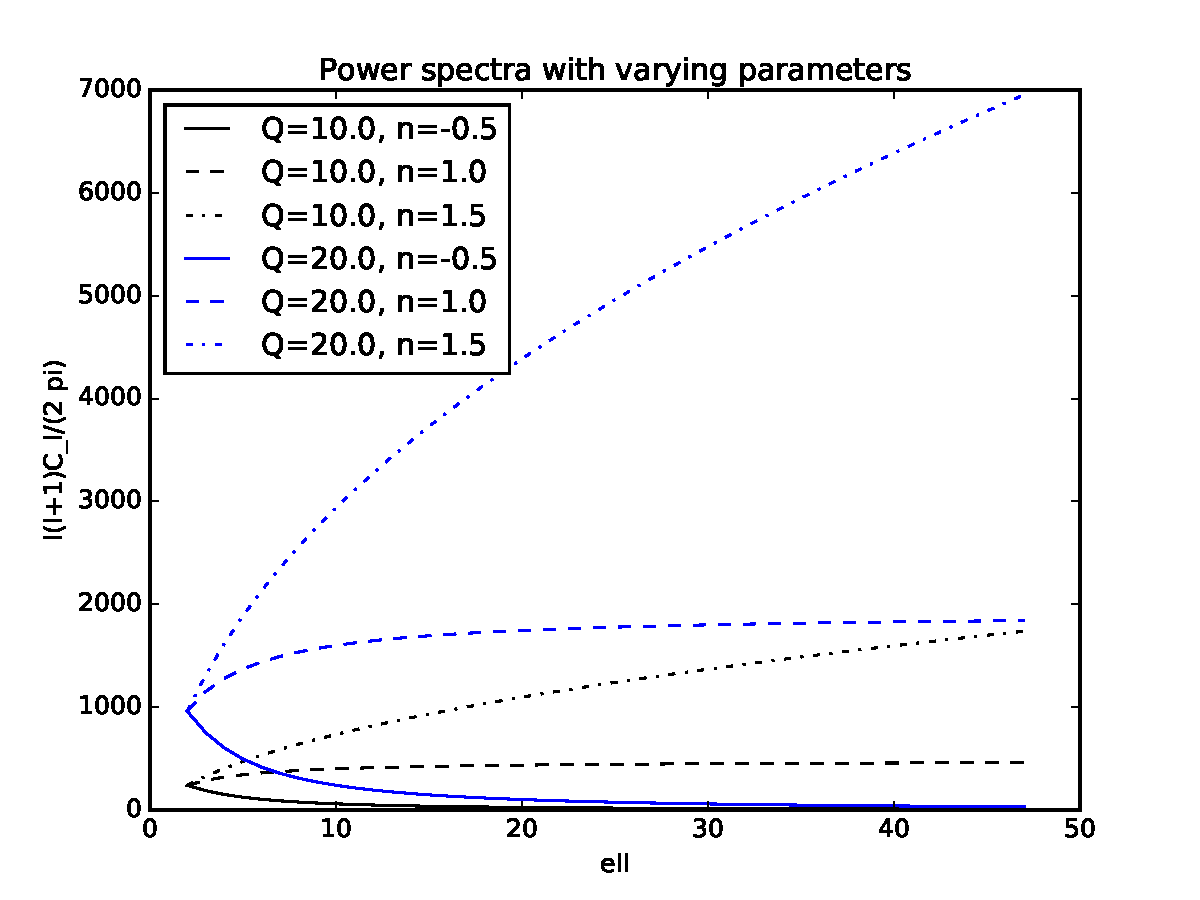
\includegraphics[width=0.7\textwidth]{cls_examples.pdf}
\caption{Angular power spectra for different values of $Q$ and $n$. \label{fig:cls}}
\end{figure}

Finally, we have to include a term that removes the effect of a possible
monopole or dipole in our maps. First of all, DMR is a so-called
differential experiments, which means that it only measures the
\emph{difference} between two points on the sky, never their absolute
values. It is therefore impossible to say what the true monopole
is. (On the other hand, this is what COBE-FIRAS did, by comparing the
sky to an internal controlled load on the satellite.) Second, it is
also impossible to measure the true cosmological CMB dipole: Earth's
motion through space results in a Doppler shift of the CMB monopole,
which takes the form of a dipole. The observed dipole is therefore
only a reflection of our motion, rather than a cosmologically
interesting quantity.

To account for these terms, we should \emph{marginalize} over the
amplitude of these two modes, such that the final answers are
independent of their true values. One way to do this is to add another
term to the covariance matrix with ``infinite''
variance,
\begin{equation}
\mathbf{F} = \lambda \mathbf{f f}^{t}.
\end{equation}
where $\lambda$ is a numerically large constant (e.g., $10^3$), and
$\mathbf{f}$ is the known structure (or template) on the sky 
one wants to be insensitive to. $\mathbf{f f}^{t}$ is the
outer-product o this template with itself. Thus, if you want to
marginalize\footnote{Marginalization means to remove one variable
  from a common distribution by integrating over it. If we have a
  joint distribution $f(x,y)$, and wants to find the distribution for
  $x$ alone, we can marginalize over $y$, which means to integrate
  over all possible values of $y$: $f(x) = \int f(x,y)\,dy$} over
the monopole, you simply add a large constant to the total covariance
matrix. 

To summarize, the final covariance matrix is given by 
\begin{equation}
\mathbf{C}(Q,n) = \mathbf{S}(Q,n) + \mathbf{N} + \mathbf{F},
\end{equation}
where the three individual covariance matrices are given as above.

\subsection{Maximum likelihood analysis}

Our main goal in this project is to determine the best-fit values of
the parameters , $Q$ and $n$, given the COBE-DMR observations. There
are several methods for doing so, but we will adopt the so-called
\emph{maximum-likelihood} framework. 

The likelihood function is defined simply as,
\[
\mathcal{L}(Q,n) = p(\mathbf{d}|Q,n).
\]
This function quantifies the probability of obtaining some data set,
given the true cosmological parameters. Of course, the data are given
once and for all, so our task is not to change the data as such, but
rather ask which parameters are most likely given those data.

The joint distribution above is given by the multi-variate Gaussian
described in Equation \ref{eq:multigauss}, with the data vector
$\mathbf{d}$ as its variable. Having constructed the covariance
matrix, the rest of the analysis is fairly straightforward. Based on
this distribution, the {\em log-likelihood} reads
\begin{equation}
\label{eq:lnL}
-2\log \mathcal{L}(Q,n) = \mathbf{d}^T \mathbf{C}^{-1} \mathbf{d} +
\log |\mathbf{C}| + \textrm{constant},
\end{equation}
and our task is to evaluate this for different values of $(Q,n)$. 

Note that it is usual to consider the log-likelihood rather than the
likelihood itself, since this is a numerically more well-behaved
number. With 1000 pixels, the log-likelihood will typically have
values of order 1000, while the likelihood itself will be
$\mathcal{O}(e^{-1000})$. Numerical errors quickly become difficult to
handle. It is therefore a very good tip to perform all calculations in
log units, and only exponentiate at the very end. You can also
disregard any constants in the log-likelihood, since this corresponds
just to a normalization factor, which you can reconstruct in the end
by requiring that the final function should have integral equal to
one. 

The main product in this project is thus a two-dimensional contour
plot of the likelihood evaluated for $(Q, n)$. In our particular case,
the data set is small enough that brute-force grid evaluation is
feasible even on a laptop. However, for larger data sets or more
sophisticated models, Markov Chain Monte Carlo methods may be
preferable. If you want to, you can of course solve the current
problem using this method, which is both fun and instructive.

After calculating the two-dimensional likelihood, you must also
compute the one-dimensional marginal best-fit values for each
parameter individually, with associated uncertainties. Mathematically,
you obtain the distribution for one parameter by integrating over the
other, 
\begin{equation}
\mathcal{L}(Q) = \int \mathcal{L}(Q,n) dn.
\end{equation}
If you choose MCMC, this task is trivial, since you then simply can
make a one-dimensional histogram from the samples directly. If you
perform the mapping by 2D gridding, you actually have to perform the
integral numerically. In both cases, you want to derive an answer on
the form $n = 1.1\pm0.2$.

\subsection{Implementation}

In principle, you are completely free to implement this project in
whatever computer language you want. However, the simplest solution is
clearly to use the Python template that is made available in the
standard directory. This template is a close to complete version of
the final program, with only a few critical lines removed. 


The program consists of two files, namely the main program
(``cmb\_likelihood.py'') and a utility module
(``cmb\_likelihood\_utils.py''). The main program is complete, and you
don't have to do anything with this, unless you want to. But you
definitely need to read through it, and make sure you understand what
happens at the various places. Furthermore, if you want to output the
final results in another format than the default, you have to do this
in the main program.

The utility module is however not complete. All subroutines are in
place, but the most critical lines are missing. What actually is
missing is listed in the beginning of the module. This is also marked
in each routine, although not necessarily how it should be done.

% Makefiler er allerede satt opp, slik at koden skal kunne kompileres p�
% en hvilken som helst alpha-maskin p� instituttet ved kommandoen
% ``make''.

\subsubsection{Programming tips}

There are two operations in this project that may turn out very
time-consuming, at least if you use Python. For these, it is important
to implement the codes in a clever way. This concerns the evaluation
of the signal covariance matrix $\mathbf{S}$ (Equation \ref{eq:S}) and
the final log-likelihood (equation \ref{eq:lnL}).

\paragraph{Covariance matrix:}

Given the expression for $\mathbf{S}$ it is easy to set up a triple
for-loop to evaluate this matrix. However, this is very slow in
Python, and it is always a good idea to vectorize Python code whenever
possible. Fortunately, we have NumPy, which is a C-based library, that
is optimized for array operations. You therefore want to put on your
``vector glasses'' when implementing this expression: It may be
considered as a series of element-wise vector multiplications followed
by one inner product, corresponding to the sum over $\ell$. You should
try both methods, just to check how much faster the code runs with
vectorization, and to make sure they give the same answer, for
debugging purposes. 

\paragraph{Log-likelihood:}

The expression for $\log\mathcal{L}$ also suggests an obvious solution
strategy: Invert $\mathbf{C}$ with, say, scipy.linalg.inv, and then
compute the determinant with for instance scipy.linalg.det or
numpy.linalg.slogdet. Matrix inversion and determinant evaluation are
however expensive operations, and fortunately people have worked on
this before us, and there are today fast libraries for such
operations, such as LAPACK. However, it is actually quite rare that
one needs to actually invert a covariance matrix, as one can often use
what is called a Cholesky decomposition instead. 

The Cholesky decomposition is a product of a triangular matrix with
its own transpose
\[
\mathbf{A} = \mathbf{L}\mathbf{L}^{\mathrm{T}}\quad \Rightarrow \quad \mathbf{A}^{-1} = (\mathbf{L}^{-1})^{\mathrm{T}}\mathbf{L}^{-1}.
\]
With this decomposition, the determinant is essentially free, since
one has
\[
\det\mathbf{A} = \det\mathbf{L}\,\det(\mathbf{L}^{\mathrm{T}}) = (\det\mathbf{L})^2,
\]
since the determinant of a triangular matrix is just to product over
all diagonal elements.

Solving an equation set on the form
\[
\mathbf{L}\mathbf{x} = \mathbf{y}
\]
for $\mathbf{x}$ is very simple, and it is much faster than inverting
a matrix, even with use of LAPACK. The trick is therefore to rewrite
\[
\mathbf{d}^T \mathbf{C}^{-1} \mathbf{d}, \quad \mathrm{der} \quad \mathbf{C}^{-1} = (\mathbf{L}^{-1})^{\mathrm{T}}\mathbf{L}^{-1},
\]
to something like
\[
\mathbf{x}^T \mathbf{x},
\]
where $\mathbf{x}$ is the solution of the triangular equation set as
shown above. 

SciPy-rutinene scipy.linalg.cholesky and
scipy.linalg.solve\_triangular will be useful for this.

If you are stuck, don't hesitate to ask Hans Kristian
either in person or by email (h.k.k.eriksen@astro.uio.no): Do not
spend massive amounts of time to figure out a problem if it takes two
minutes to ask somebody else! :-)

\subsection{Data}

The required data are stored in the standard directory given in the
beginning of the project description:
\begin{itemize}
\item cobe\_dmr\_53GHz\_n16.npy(.dat)-- DMR map and RMS values for the
  53GHz channel, given in form of a list of unmasked pixel values and
  corresponding directional vectors. 
\item cobe\_dmr\_90GHz\_n16.npy(.dat)-- DMR map and RMS values for
  90GHz channel, as above
\item cobe\_dmr\_beam.npy(.dat)-- DMR beam function $b_{\ell}$, given
  for each multipole $\ell$.
\item pixwin\_n16.npy(.dat)-- Healpix pixel window at $N_{\textrm{side}}=16$.
\item params.py -- parameter file for the cmb\_likelihood program
\end{itemize}
Results should be generated and shown for both the 53 and 90 GHz
channels. 

Note that the data files are given in two equivalent formats, either
binary NumPy array files or ordinary ASCII text files. For those who
choose to do the project in Python, the first format is definitely
preferable, while the .dat files are available for those who prefer a
different language. 


\subsection{Plotting the results}

As always, how to make the contour plots is up to you. We do however
provide a very simple template that works as an example, called
``plot\_contours.py'' in the 'work' directory. This script takes the
output from the cmb\_likelihood program, and shows the corresponding
contour plot on the screen. Writing this to file, and make the figure
prettier, is your task. You can of course ask your fellow students --
or do it in a completely different way, if you prefer that. 

\section{Part 2 -- ``Publishing'' in Astrophysical Journal Letters}

The programming in this project is quite simple, and consists of
adding a few simple commands in a nearly finished program. The run
time of the code will take a few hours, perhaps a day, depending on
how many grid points you want. 

The main work load is associated with writing the paper. You should do
this in the standard format that has already been provided, using all
the tips that were given in the first few projects. 

Regarding style, imagine that you write this paper for the first time
in 1994, and not in 2016. In other words, pretend that this is the
first discovery of the CMB fluctuations. So, don't be too modest --
this will result in a Nobel prize in 15 years. Yet, use a scientific
language and style: You know that you have something really cool on
your hands, but you don't want to be annoying :-)

The paper should contain (at least) the following points:
\begin{enumerate}
\item An abstract that briefly summarizes the problem, the methods and
  the results. 
\item An introduction that provides a setting for the analysis -- why
  do we do this, what does the theory tell us, and what is the current
  status of the field?
\item A method section that describes the model (including definition
  of the covariance matrix), the likelihood, and the algorithm used to
  map the likelihood
\item Data summary: Which data are used, which frequencies, what
  angular resolution etc. 
\item Results
  \begin{enumerate}
    \item Both 53 and 90GHz maps must be analyzed
    \item 2D contour plots for each case, preferably over-plotted
    \item Best-fit one-dimensional values listed in a table, including uncertainties
    \item Details regarding the analysis  (e.g., run time) may also be
      included.
  \end{enumerate}
\item Conclusion: What has been found, and what does it imply? What
  should be done next, in order to bring the CMB field to its full
  fruition? 
\end{enumerate}


Finally, if something is unclear, wrong or needs improvement, please
don't hesitate to say so. All feedback is very much welcome :-)

\end{document}









